\section{Ejercicio 4}
En este apartado se realizar\'a el dise\~no de un circuito adaptador de se\~nal, por ejemplo para que esta pueda ser le\'ida por un microcontrolador. Para tal fin es necesario conocer tanto los par\'ametros de entrada como los de salida, as\'i como las limitaciones presentes en el dise\~no.

\subsection{Se\~nal de entrada}
La se\~nal de entrada del circuito provendr\'a de un \textsc{mpx2010dp}. Este es un sensor de presi\'on que opera de forma piezorresistiva. Esto significa que la magnitud ser\'a medida indirectamente a trav\'es de un cambio en la resistencia de un resistor calibrado. Dicha diferencia est\'a dada por una peque\~na deformaci\'on en la geometr\'ia del resistor debido a la presi\'on ejercida por un flu\'ido hidr\'aulico encapsulado en el interior del sensor propiamente dicho.

\begin{figure}[H]
    \centering
    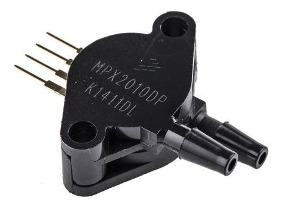
\includegraphics[width=0.5\textwidth]{../EJ4/resources/mpx2010dp.png}
    \caption{Sensor \textsc{mpx2010dp}}
    \label{fig:EJ4_mpx2010dp_image}
\end{figure}

Como se puede observar en la imagen anterior el sensor posee dos entradas de fluido. Esto es as\'i dado que el mismo mide la presi\'on de una de las entradas, en relacion a la otra. Esto es precisamente \'util para medir la presi\'on manom\'etrica de un determinado fluido (esto es, su presi\'on en relaci\'on a la atm\'osfera. De esta forma, el sensor entrega una se\~nal de tensi\'on que ser\'a lineal y proporcional a esta diferencia de presi\'on. Esto se puede observar en la figura~\ref{fig:EJ4_mpx2010dp}.

\begin{figure}[H]
    \centering
    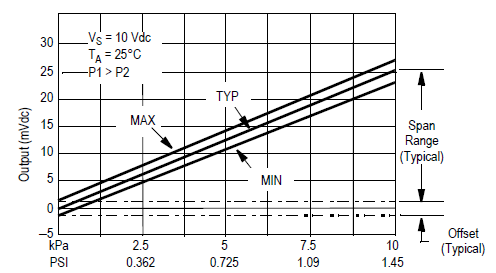
\includegraphics[width=0.5\textwidth]{../EJ4/resources/mpx2010dp_out.png}
    \caption{Salida del \textsc{mpx2010dp} en funci\'on a la diferencia de presi\'on}
    \label{fig:EJ4_mpx2010dp_out}
\end{figure}

Como se puede apreciar en la figura anterior, la salida del sensor oscila entre $0V$ y $25mV$ aproximadamente (para diferencias de presi\'on de $0KPa$ y $10KPa$ respectivamente). Este rango de tensi\'on se ubica en el orden de magnitud del piso de ruido, por lo que emplear este sensor sin amplificar resultar\'ia en mediciones err\'oneas y probablemente aleatorias (en funci\'on del tipo de ruido presente en el lugar de operaci\'on del sensor). A\'un asi realizando una amplificaci\'on de la salida hay que tener en cuenta que el circuito que se encargue de ello debe ser lo suficientemente inmune al ruido como para que la salida del mismo sea representativa de la presi\'on ejercida sobre el sensor.


Por esta raz\'on es apropiado emplear un circuito que contenga un amplificador de instrumentaci\'on, de forma tal de minimizar el error de medida a la salida. 

\subsection{Amplificador de instrumentaci\'on}

Un amplificador de instrumentaci\'on es un circuito compuesto por amplificadores operacionales y resistores que satisface los siguientes requerimientos:

\begin{enumerate}
		\item Impedancias de entrada en modo com\'un y diferencial altas (idealmente infinitas).
		\item Impedancias de salida muy bajas (idealmente nulas).
		\item Ganancia alta y relativamente estable.
		\item Alto grado de CMRR \textit{(Common Mode Rejection Ratio)}
\end{enumerate}

Estas caracter\'isticas hacen al amplificador especialmente apto para aplicaciones cuyas se\~nales sean d\'ebiles, como por ejemplo en el campo de la medicina. Tambi\'en es ideal para amlpificar el sensor \textsc{mpx2010dp}. En l\'ineas generales existen dos circuitos de instrumentaci\'on: uno que utiliza dos amplificadores operacionales y otro que usa tres.

\begin{figure}[H]
    \centering
    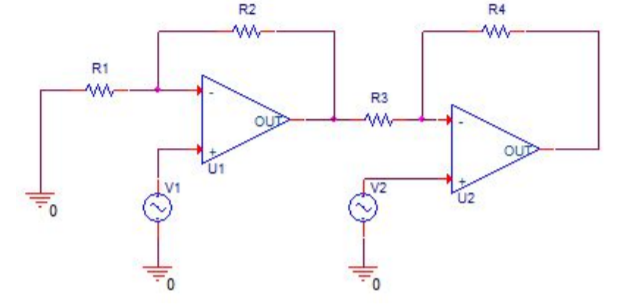
\includegraphics[width=0.9\textwidth]{../EJ4/resources/instrumental_2opamp.png}
    \caption{Amplificador de instrumentaci\'on de 2 op-amp}
    \label{fig:EJ4_instrumental_2opamp}
\end{figure}

\begin{figure}[H]
    \centering
    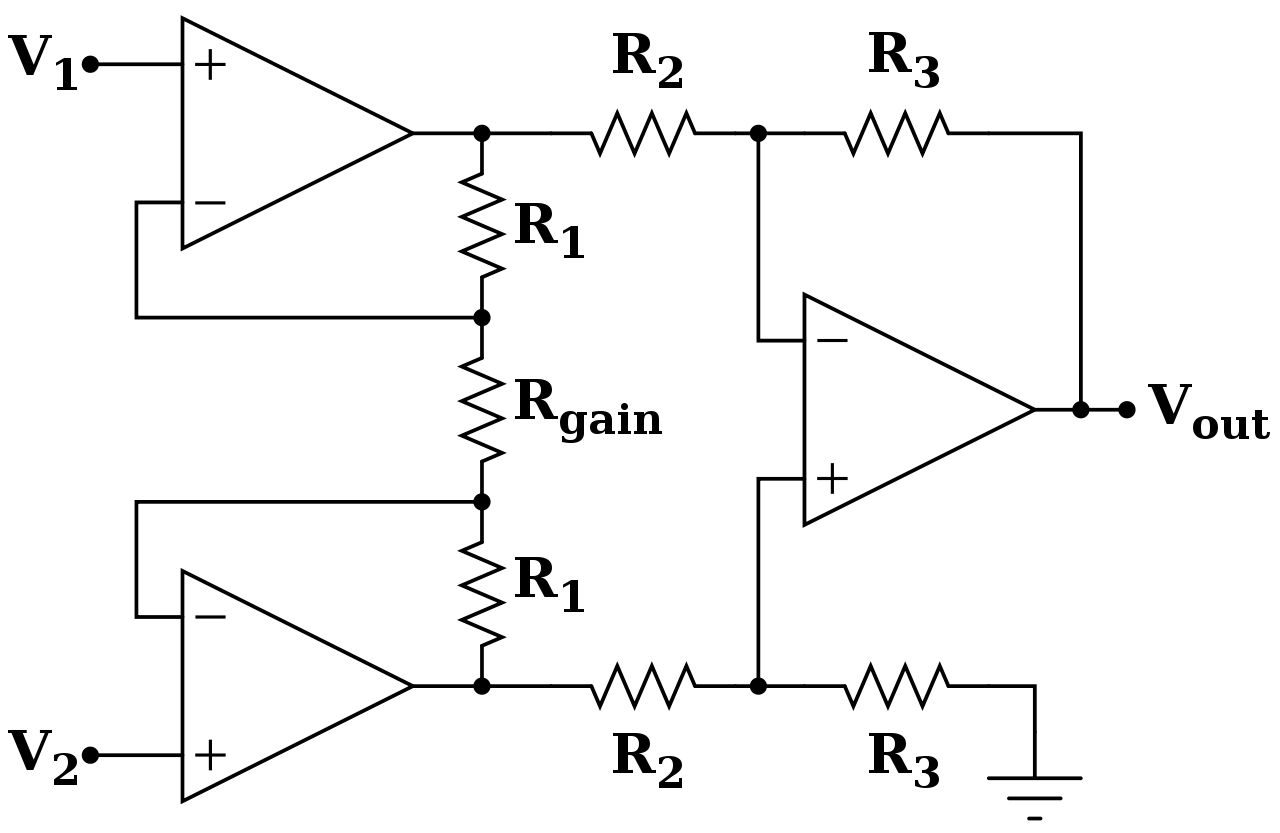
\includegraphics[width=0.9\textwidth]{../EJ4/resources/instrumental_3opamp.png}
    \caption{Amplificador de instrumentaci\'on de 3 op-amp}
    \label{fig:EJ4_instrumental_3opamp}
\end{figure}
 
 La principal ventaja de la configuraci\'on dual es que obviamente se requieren menos amplificadores operacionales. Por otro lado, comparado con la configuraci\'on de tres op-amp el circuito tratar\'a a las dos entradas ($v_1$ y $v_2$) de forma asim\'etrica, debido al tiempo de propagaci\'on existente entre las dos etapas. Este factor hace que el coeficiente de CMRR se degrade en rango de frecuencias elevado. Esta variable no afecta al diseño, dado que se trabaja con tensi\'on en corriente continua y constante. Explicado esto, se utilizar\'a la configuraci\'on de op-amp dual.
 
 
Para este circuito se realiza un an\'alisis de forma tal de conseguir la ganancia del sistema. Para ello se modelizan las entradas en modo diferencial como dos fuentes de valor $\frac{v_d}{2}$ y una tensi\'on $v_{cm}$ que simboliza una componente presente en ambas entradas de igual forma, que por ejemplo puede ser la representaci\'on de ruido en las se\~nales. El modelo se presenta a continuaci\'on.

\begin{figure}[H]
    \centering
    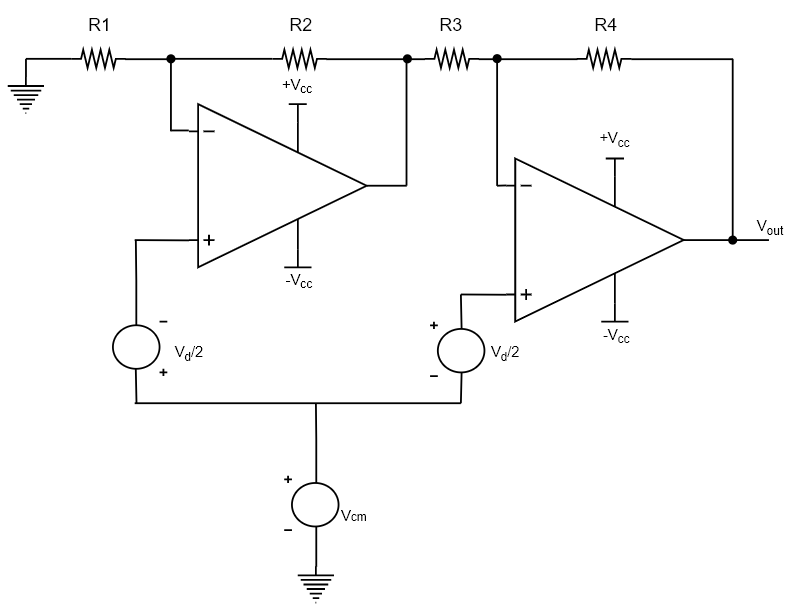
\includegraphics[width=0.9\textwidth]{../EJ4/resources/2opamp_difmode_gain.png}
    \caption{C\'alculo de ganancia en modo diferencial}
    \label{fig:EJ4_2opamp_difmode_gain}
\end{figure}

Si se aplica el principio de superposici\'on sobre las dos entradas no inversoras de los amplificadores operacionales se obtiene la siguiente ecuaci\'on, que refleja la ganancia en modo diferencial del sistema, en funci\'on de los resistores que lo componen.

\begin{equation}
V_{out} = \frac{v_d}{2} \cdot \left( 1 + \frac{2R_4}{R_3} + \frac{R_2 \cdot R_4}{R_1 \cdot R_3} \right) + v_{cm} \cdot \left( 1 - \frac{R_2 \cdot R_4}{R_1 \cdot R_3} \right)
\label{EJ4_vout}
\end{equation}

En la ecuaci\'on anterior se pueden distinguir dos t\'erminos: por un lado, uno dependiente de $v_d$ (que es la se\~nal que se busca amplificar), y por otro uno dependiente de $v_{cm}$ cuyo impacto se busca minimizar. Para lograr esto \'ultimo, se puede asumir una condici\'on de puente entre los resistores,  lo que deriva en la siguiente equivalencia.

\begin{equation}
\frac{R_1}{R_2} = \frac{R_4}{R_3} 
\label{EJ4_condicion_puente}
\end{equation}

De esta forma, se simplifica la expresi\'on de la ecuaci\'on~\ref{EJ4_vout} y se obtiene

\begin{equation}
v_{out} = v_d \cdot \left( 1+\frac{R_1}{R_2} \right) = v_d \cdot \left( 1+\frac{R_4}{R_3} \right
\end{equation}

Luego, seleccionando los valores de dos resistores se fija la ganancia del sistema. Dado que los valores de resistencia se encuentran normalizados, y que el rango de se\~nal entregado por el sensor puede variar en un rango determinado por el fabricante, es necesario contar con una ganancia ajustable, para poder realizar una calibraci\'on del circuito de forma tal de que funcione como fue pensado.


En  este sentido se cuenta con el problema de que no es posible variar un solo resistor, dado que se deber\'ia ajustar simult\'aneamente otro resistor, para poder satisfacer la condici\'on de puente expresada en la ecuaci\'on~\ref{EJ4_condicion_puente}. De esta forma, se propone el siguiente circuito, que es capaz de ajustar la ganancia sin afectar la condici\'on de puente antes mencionada.


\begin{figure}[H]
    \centering
    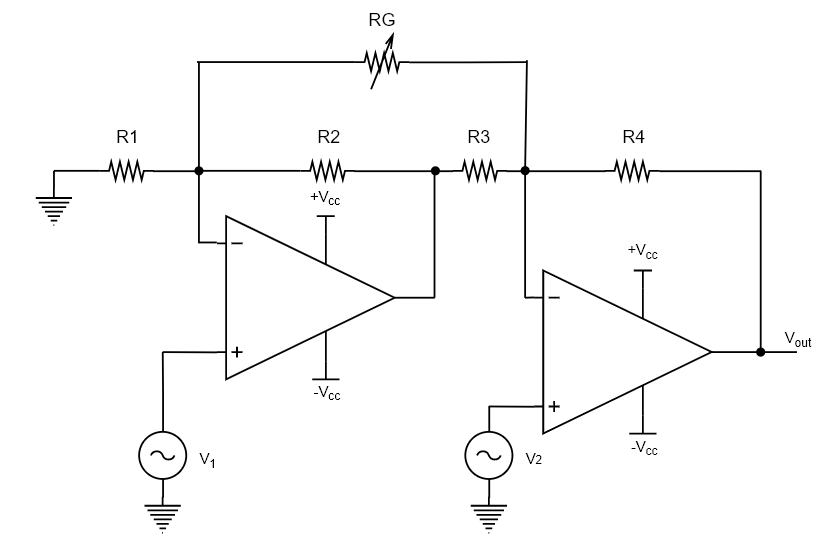
\includegraphics[width=0.9\textwidth]{../EJ4/resources/instrumental_2opamp_adjgain.png}
	\caption{Amplificador de instrumentaci\'on con ganancia ajustable}
   	\label{fig:EJ4_2opamp_adjgain}
\end{figure}

Del circuito anterior se deduce la ganancia, seg\'un la siguiente ecuaci\'on:

\begin{equation}
v_{out} = v_d \cdot \left( 1+\frac{R_2}{R_1}+\frac{2R_2}{R_G} \right)
\label{EJ4_adjgain}
\end{equation}

De esta forma, la ganancia tendr\'a una dependencia no lineal respecto de la resistencia variable $R_G$.

\subsection{Selecci\'on de componentes}

Se deben seleccionar los componentes para obtener la ganancia deseada. De la datasheet del circuito se observa que el rango de tensiones de salida del sensor \textsc{mpx2010dp} va desde $0V$ a $25mV$. La salida del circuito debe ser de $0V$ a $3,3V$. Luego, la ganancia te\'orica del sistema debe valer $A = 66$. De la ecuaci\'on~\ref{EJ4_adjgain} se deduce la siguiente igualadad.


\begin{equation}
A = 1+\frac{R_2}{R_1}+\frac{2R_2}{R_G}
\end{equation}

Con la expresi\'on anterior, y fijando $R_2$ y $R_1$ a valores normalizados, se obtiene la siguiente combinaci\'on de componentes.

\begin{table}[H]
    \centering
    \begin{tabular}{c c c c}
        $R_1 = R_4$ & $R_2 = R_3$ & $R_G$ & $Preset (R_G)$  \\
        \hline \\
        $68 K\Omega$ & $82 K\Omega$ & $2.57 K\Omega$ & $5 K\Omega$ \\
        \hline
    \end{tabular}
\end{table}

En general se busca utilizar componentes SMD dado que las tolerancias son del $1\%$, por lo que tendr\'an menos impacto sobre la condici\'on de puente. Para el resistor $R_G$ se utilizar\'a un preset de forma tal de hacer la ganancia ajustable.

\subsection{Limitaci\'on del rango de salida}

Dado que el circuito adapta se\~nales que pueden ser utlizadas por ejemplo por un microcontrolador, es necesario limitar la salida del mismo a un valor seguro para la etapa que adquiere la se\~nal. En este caso, el l\'imite superior de la salida est\'a dentro del rango comprendido entre $3,1V$ y $3,3V$. Para ello, se puede emplear un diodo zener en paralelo a la salida del circuito. Para ello se seleccion\'o un diodo cuyo valor de tensi\'on de zener asciende a $v_z = 3,3V$.


En este punto cabe destacar que al accionarse esta protecci\'on hay que tener especial cuidado en la corriente que se le exige a los amplificadores operacionales, debido a que es factible que el valor sea excesivo, haciendo que el circuito se queme. Para evitar esto, se puede colocar una impedancia en serie a la salida del \'ultimo amplificador operacional, de forma tal de limitar la corriente.


Para realizar el c\'alculo de la corriente m\'axima admisible por el integrado se busca de la datasheet del operacional que el DC Swing m\'aximo a la salida es de $\pm 13,5V$, cargando al circuito con una impedancia de $10k\Omega$. Esto resulta en una intensidad m\'axima de $13,5mA$, y aplicando un coeficiente de margen se emplea $I_{out}^{max} = 10mA$.

Con la corriente m\'axima calculada, y suponiendo que la m\'axima salida del sensor es $26mV$ (dato proveniente de la hoja de datos), se deduce que la salida del circuito presentar\'a una tensi\'on de aproximadamente $3,432V$. Si a esto se le resta la ca\'ida en el zener, y dividiendo por la corriente m\'axima deseada se obtiene:

\begin{equation}
R_z = \frac{\Delta V_{R_z}}{I_{max}} = 13,2 \Omega
\end{equation}

Normalizando el valor, se utiliza un resistor de valor $R_z = 13,2 \Omega$.

Cabe resaltar que otra opci\'on factible para limitar la salida del circuito es utilizar un amplificador operacional del tipo rail to rail, aliment\'andolo con una tensi\'on dentro del rango de tensi\'on de salida m\'axima. Esto fue desestimado en principio porque el circuito debe tener una sola alimentaci\'on, y se considrer\'o que el sensor de presi\'on requiere un valor m\'as alto para funcionar correctamente. Por otro lado, el integrado que contiene a los amplificadores con estas caracter\'isticas tiene un costo mayor.

\subsection{Simulaci\'on del circuito}

Habiendo realizado el dise\~no y el c\'alculo del circuito, se procede a realizar las simulaciones pertinentes para verificar que este funcione correctamente. Particularmente, se llev\'o a cabo un an\'alisis montecarlo para poder observar c\'omo afecta la tolerancia de cada uno de los componentes al comportamiento del amplificador. Todos los resistores son del tipo SMD, y poseen una tolerancia del $1\%$. Se asume al circuito calibrado por el preset, cuya tolerancia es supuesta nula debido a que es ajustable. A continuaci\'on se adjunta la simulaci\'on.

\begin{figure}[H]
    \centering
    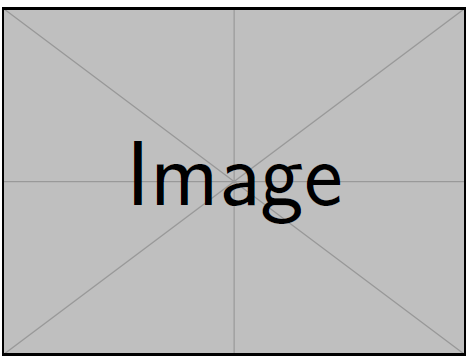
\includegraphics[width=0.9\textwidth]{../EJ4/resources/montecarlo.png}
	\caption{Montecarlo del circuito}
   	\label{fig:EJ4_montecarlo}
\end{figure}


\subsection{Medici\'on de volumen}

El circuito sintetizado anteriormente puede ser adaptado para medir el volumen de l\'iquido contenido en un tanque cil\'indrico de radio conocido.

Se observa que la presi\'on se define como $P = \frac{\Delta F}{\Delta S}$, donde $F$ es la fuerza ejercida sobre una superficie de \'area $S$. Como el origen de esta fuerza es el peso de un l\'iquido de densidad $\delta$, entonces $F = \delta \cdot h \cdot A$ (donde $h$ representa la altura de columna de l\'iquido). Si combinamos estas ecuaciones se obtiene lo siguiente:

\begin{equation}
P  = \delta \cdot h
\end{equation}

Adem\'as el volumen de l\'iquido puede ser expresado como $V = S \cdot h$, por lo que el volumen tambi\'en puede ser calculado como

\begin{equation}
V = \frac{P \cdot S}{\delta}
\end{equation}

Y por otro lado se conoce la dependencia de la tensi\'on de salida respecto a la diferencia de presi\'on medida por el sensor.

\begin{equation}
v_{out} = A_{sensor} \cdot A_{circuito} \cdot P
\end{equation}

Dado que se conoce el valor del radio del recipiente y la densidad del l\'iquido que contiene, el volumen que ocupa el l\'iquido es directamente proporcional a la presi\'on que este ejerce sobre el fondo del recipiente. Luego, no habr\'ia que hacer ning\'un tipo de cambio al circuito, dado que si se conoce la tensi\'on $V_out$ se puede calcular el volumen que ocupa empleando la siguiente ecuaci\'on:

\begin{equation}
V = \frac{v_{out} \cdot S}{\delta \cdot A_{sensor} \cdot A_{circuito}}
\end{equation}

Por \'ultimo, el tanque es cili\'indrico de radio $R$ por lo que $S = \pi \cdot R^2$. Luego:

\begin{equation}
V = \frac{v_{out} \cdot \pi \cdot R^2}{\delta \cdot A_{sensor} \cdot A_{circuito}}
\end{equation}

Donde $A_{circuito} = 66$, $A_{sensor} = 2,5 \frac{mV}{KPa}$. De esta forma, el circuito podr\'a medir vol\'umenes que van desde $V_{min} = 0$ hasta $V_{m\'ax} = \frac{3,3 [Volt] \cdot \pi \cdot R^2}{\delta \cdot A_{sensor} \cdot A_{circuito}}$

Desde el punto de vista constructivo, para que lo anteriormente desarrollado sea v\'alido, una de las salidas del sensor debe estar colocada en el fondo del tanque y la otra debe estar en contacto con la atm\'osfera para actuar de referencia. De esta forma el sensor mide la presi\'on ejercida exclusivamente por la columna de agua encima de \'el (presi\'on manom\'etrica).

\subsection{Mediciones y an\'alisis}

\begin{equation}
 COMPLETAR ESTO!!!!!!!!!!!!!!!!!!!!!!
\end{equation}


%\begin{figure}[H]
%    \centering
%    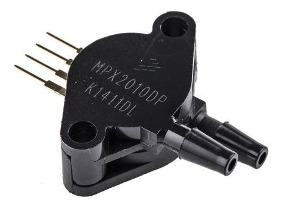
\includegraphics[width=0.9\textwidth]{../EJ4/resources/mpx2010dp.png}
%	\caption{Circuito l\'ogico}
%    \label{fig:ej4_circuito_logico}
%\end{figure}